\documentclass[a4paper,12pt]{article}
\usepackage{amssymb}
\usepackage{amsfonts}

% Кодировка и язык
\usepackage[utf8]{inputenc}
\usepackage[T2A]{fontenc}
\usepackage[russian]{babel}


% Математические пакеты
\usepackage{amsmath,amsfonts,amssymb}
%Таблицы
\usepackage{array}
\usepackage{booktabs} % Для более красивых горизонтальных линий в таблицах
\usepackage{graphicx}
\usepackage{array}
\usepackage{booktabs}
% Геометрия страницы
\usepackage{geometry}
\geometry{top=2cm, bottom=2cm, left=2.5cm, right=2.5cm}
% Гиперссылки (лучше загружать последним)
\usepackage{hyperref}


% Настройки заголовка
\title{Домашнее задание}
\author{Студент: \textbf{Ростислав Лохов}}
\date{\today}

\begin{document}

% Титульный лист
\begin{titlepage}
    \centering
    \vspace*{1cm}

    \Huge
    \textbf{Домашнее задание}

    \vspace{0.5cm}
    \LARGE
    По курсу: \textbf{Экономика}

    \vspace{1.5cm}

    \textbf{Студент: Ростислав Лохов}

    \vfill

    \Large
    АНО ВО Центральный университет\\
    \vspace{0.3cm}
    \today

\end{titlepage}

% Содержание
\tableofcontents
\newpage

% Основной текст
\section{Сине-Красный уровень}


\subsection{Задача 1}
\begin{enumerate}
    \item Монополия (несовершенная конкуренция) т.к спрос убывает с ростом обьема, что характерно для рынков, где фирма влияет на цену
    \item Максимум прибыли будет при равных предельная выручка и предельные издержки
    \item $TR = PQ = (36-4Q)Q = 36Q-4Q^2$
    \item $MR = TR' = 36-8Q$
    \item $MC = 2Q+6$
    \item $Q = 3 \rightarrow P = 24$пр
\end{enumerate}

\subsection{Задача 2}
\begin{enumerate}
    \item Фирма находится в условиях совершенной конкуренции, т.к цена равняется предельной выручке, также цена не зависит от кол-ва выпускаемой продукции.
    \item Максимальная прибыль находится в точке MR=MC, VC=4000 по условию. Прямоугольник обозначает прибыль = 1500.
    \item $\pi = 1500, \quad TR=PQ$
    \item $TR = 8000, TC = TR - \pi = 8000 - 1500 = 6500$
    \item $FC = TC - VC = 6500 - 4000 = 2500$
    \item Переменные издержки 4000 в этой точке, обьем 1000, AVC = 4, Значит по оси ординат голубая точка будет 4.
    \item Из  пересечения P и MC, TC = 6500. ATC = 6,5. Значит зеленая точка 6.5
\end{enumerate}

\subsection{Задача 3}
\begin{enumerate}
    \item $HHI = 25.52^2 + 14.68^2 + 10.22^2 + 8.5^2 + 5.16^2 + 4.98^2 + 3.93^2 + 3.82^2 + 2.73^2 + 7.45^2 =1357$
    \item После банкротства: Доля банкротства $25.52 + 14.68 = 40.2$ Новый HHI $2160$
    \item Рост HHI ухудшает конкуренцию - негативно для общества/
    \item Олигополия - власть над рынком нескольких
    \item Сокращение перевозок увеличивает прибыль, следовательно $MR < MC$
\end{enumerate}

\subsection{Задача 4}
\begin{enumerate}
    \item $AVC = \frac{VC}{Q}, MC = TC'$
    \item При субсидировании происходит уменьшение издержек, кривая издержик снизится на велиину субсидии.
    \item Поскольку фирма работает в условиях совершеной конкуренеции, цена находится на уровне рынка. Т.к затраты уменьшились, то происходит больше товаров, а значит кривая предложения смещается вправо.
\end{enumerate}

\subsection{Задача 5}
\begin{enumerate}
    \item $MC = VC' = 4Q+20$
    \item $120 = 4Q + 20 \Rightarrow Q = 25$
    \item $\pi = TR - TC = 120*25 - (2*25^2+20*25+1000)=250$
\end{enumerate}

\subsection{Задача 6}
\begin{enumerate}
    \item $MR = TC$
    \item $MC = Q + 2$
    \item $10-Q=Q+2 \Rightarrow Q = 4$
    \item $P = 10-0.5*4=8$
    \item $\pi = 8*4-(0.5*4^2+2*4+5)=11$
    \item Индекс Лернера: $L = \frac{P-MC}{P}=0.25$
\end{enumerate}

\section{Черный уровень}
\subsection{Задача 1}
\begin{enumerate}
    \item Отсутствие отечественных аналогов, после роста цен спрос не изменился, т.е монополия или олигополия, после выхода новых производителей рынок перешел в олигополию
    \item 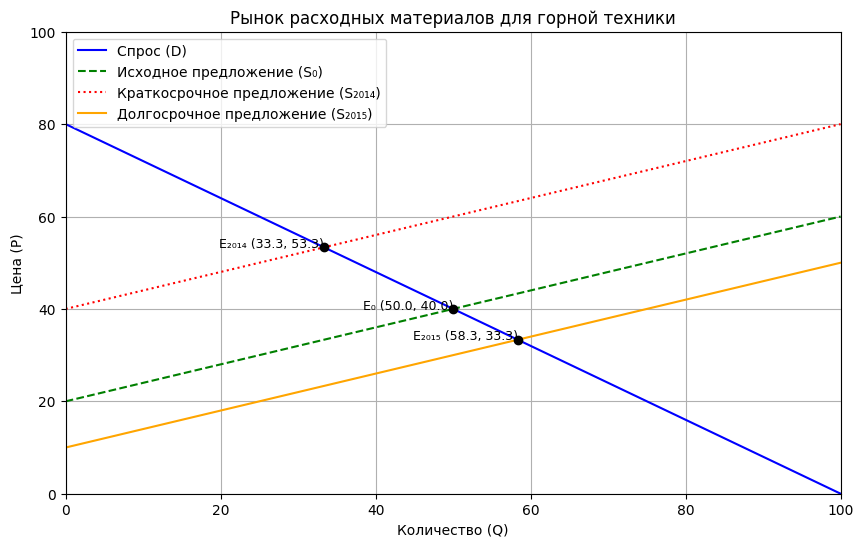
\includegraphics[scale=0.5]{graphs/7.1.png}
    \item Эластичность спроса - неэластичная, т.к при резком росте цен спрос не сократился(отсутствие заменителей, критическая важность расходных материалов для работы техники)
\end{enumerate}

\subsection{Задача 2}

\begin{enumerate}
    \item $Q = 2, \Rightarrow AC = 4$
    \item В монополии цена равна средним издержкам и предельный доход равен предельным издержкам.
    \item $P=AC=4$
    \item $A=a-bP \Rightarrow 2 = a-4b$
    \item $TC=ACQ=Q^3-5Q^2+10Q \Rightarrow MC = TC'=3Q^2-10Q+10$
    \item $MC = 3*2^2-10*2+10=2$
    \item $P=\frac{a-Q}{b}$
    \item $TR = PQ = \frac{aQ-Q^2}{b} \Rightarrow MR = \frac{a-2Q}{b}$
    \item $MR = MC \Rightarrow \frac{a-4}{b}=2$
    \item $\frac{-2+4b}{b}=2 \Rightarrow -2+4b=2b \Rightarrow 2b = 2 \Rightarrow b = 1$
    \item $Q=6-P$
\end{enumerate}

\subsection{Задача 3}

\begin{enumerate}
    \item Альтернативные издержки производства Шила: Предприятие Г: 32 руб./тыс. шт. Предприятие В: 44 руб./тыс. шт. Предприятие Б: 48 руб./тыс. шт. Предприятие А: 50 руб./тыс. шт.
    \item Оптимальный объём Шила: Производить шило, пока $MR \ge MC$
    \item Для предприятия Г: Q=10 тыс. шт., MR = 80 (выше MC = 32).
    \item Для предприятия В: Q=9 тыс. шт., MR = 44(равно M C = 44).
    \item Распределение: Шило: Г 10 тыс, В - 9тыс. Итого 19 тыс шт.
    \item Распределение: Мыло: 150 120 11 0 - А Б В Г соответственно
    \item Выручка: шило: 1558000р, Мыло: 1124000р  сумма - 2682000
    \item Прибыль: $2682000 - 2000000 = 682000$
\end{enumerate}
\end{document}
